\section{Projektstyring}
\subsection{Scrum}
Vi har anvendt \textit{Scrum} som værktøj til projektstyring igennem hele forløbet med hovedopgave. Det giver nogle gode retningslinjer for hvordan man skal planlægge et projekt, og giver samtidig mulighed for nemmere at forhindre at ens projekt går i den forkerte retning. I forlængelse af at man typisk vil prøve at undgå fejl eller dårligere perioder samt dårlig arbejdsgang, giver \textit{Scrum} også mulighed for at rette op på de ting der går skidt eller hvis man er utilfreds med noget.

\subsection{Planlægning}
Vores projekt er delt op i nogle perioder, som kaldes for et \textit{sprint}. Et sprint varer for vores vedkommende 2 uger, og består af nogle forskellige faser.
Det starter med \textit{sprint planning}, som er den fase hvor vi planlægger hvad vi skal lave af opgaver inden for sprintet. Vores overordnede opgaver for projektet er beskrevet i en \textit{backlog}, som er defineret ud fra use cases. Fra \textit{backlog'en} trækker vi de opgaver ind i det kommende \textit{sprint}, som vi mener er mulige at lave færdige inden tidsperioden på to uger er gået. Efter de overordnede opgaver er trukket ind i \textit{sprintet}, skal de deles op i mindre og mere håndtèrbare opgaver. Når dette er gjort og vi er enige om hvad opgaven indeholder, kaster vi nogle point på de opdelte opgaver som definerer hvor lang tid vi tror det tager at løse det givne problem. Så snart vi er enige om hvor tidskrævende alle opgaver er, kan \textit{sprintets} største fase begynde hvor vi løser opgaver.
\\\\
Hver dag starter med et \textit{daily stand-up} møde, hvor hver medlem af gruppen fortæller om hvad personen lavede dagen før, hvad der skal laves den pågældende dag og eventuelt hvilke udfordringer der har været eller hvis man har noget vigtigt der skal drøftes.
\\\\
Når et \textit{sprint} er overstået holdes der \textit{sprint review}, hvor vi inviterer interessenter til et møde der går ud på at fremvise hvad vi har lavet i løbet af det forgange \textit{sprint}. På mødet er det også muligt for andre at komme med feedback til produktet eller arbejdsgangen.
\\\\
Til \textit{sprint retrospective} reflekterer vi blandt andet over \textit{sprintets} forløb og konkluderer på feedback. Herefter nedskriver hvert medlem af gruppen et tal fra 1-5, hvor 1 er lavest og 5 er højest. Dette tal summerer op hvor godt man personligt har haft det i løbet af sprintet. Til tallet følger der nogle positive og negative kommentarer, som er en forklaring på det tal hver person er endt med. Vi taler herefter frit fra leveren om de gode og dårlige oplevelser i løbet af sprintet, og så sørger gruppens \textit{scrum master} for at eventuelle bliver løst.
\\\\
Vi har tilføjet en graf der viser det gennemsnitlige humør-tal uge for uge. Den afspejler hvor godt gruppen synes forløbet er gået.
\\\\
TODO: Indsæt happiness graf (sprint 1: 4, sprint 2: 3, sprint 3: 4 )
\subsection{Scrum værktøjet YouTrack}
I projektperioden har vi anvendt YouTrack til at visualisere metoder fra Scrum.
\\
Selvom vi har anvendt andre værktøjer på studiet og i praktikken, faldt valget på YouTrack, da dette værktøj er gratis og
har givet os nødvendig funktionalitet, for at kunne planlægge opgaver og holde styr på deres stadier.
\\\\
YouTrack giver mulighed for at lave rapporter, hvor vi kun har brugt muligheden for at lave et burndown chart. Herudover kan man oprette
en backlog og et sprint. Herefter har man mulighed for at opdele sine backlog opgaver og trække dem ud i en såkaldt \textit{swim lane}, der har forskellige
stadier, \textit{Open}, \textit{In Progress}, \textit{Fixed}, \textit{Verified}. På denne måde kan vi hele tiden opdatere hvor langt i processen vi er nået
med de enkelte opgaver, og få et overblik over hvad medlemmerne i gruppen laver eller hvad der mangler at blive lavet i det nuværende sprint.
\\
En mangel i Youtrack har været at vi ikke har haft mulighed for at lave en projekt backlog. Denne bruges typisk til at indeholde de overordnede opgaver i
projektet som mangler at blive lavet. Da vi følte det nødvendigt at have en sådan backlog, har vi selv valgt at lave et dokument på Google Docs, og gjort det tilgængeligt
for begge gruppens medlemmer. Dette dokument bruges til at skabe et overblik over hvilke overordnede opgaver vi har tilbage i projektet, samt tilføje nye opgaver der kan opstå.
Listen er delt op i opgaver til det konkrete system og vores rapport, og hver gang vi har skulle planlægge nye sprints, har vi taget opgaver fra vores projekt backlog over i
det enkelte sprints backlog.
\\\\
Vi har nedenfor tilføjet nogle reelle eksempler fra vores projektperiode, af et burndown chart, en swim lane med opdelte opgaver fra backlog'en og vores projekt backlog.
\\\\
TODO: Tilføj billeder af et burndown chart, en swimlane og vores projekt backlog. (Ligger på google docs)
\begin{figure}[here]
    \makebox{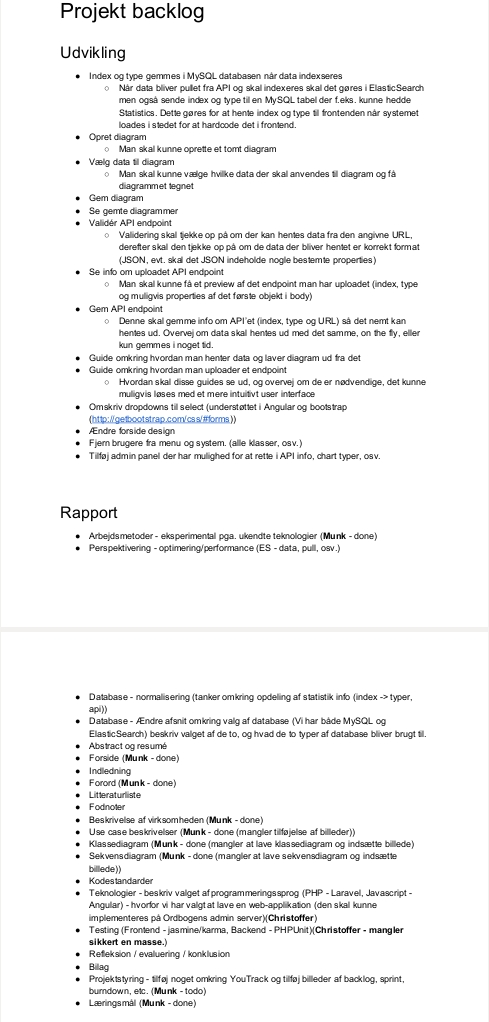
\includegraphics[scale=0.75]{Projekt_backlog}}
    \caption{Vores projekt backlog dokument}
    \label{fig:projekt-backlog}
\end{figure}
\begin{figure}[here]
    \makebox[\textwidth]{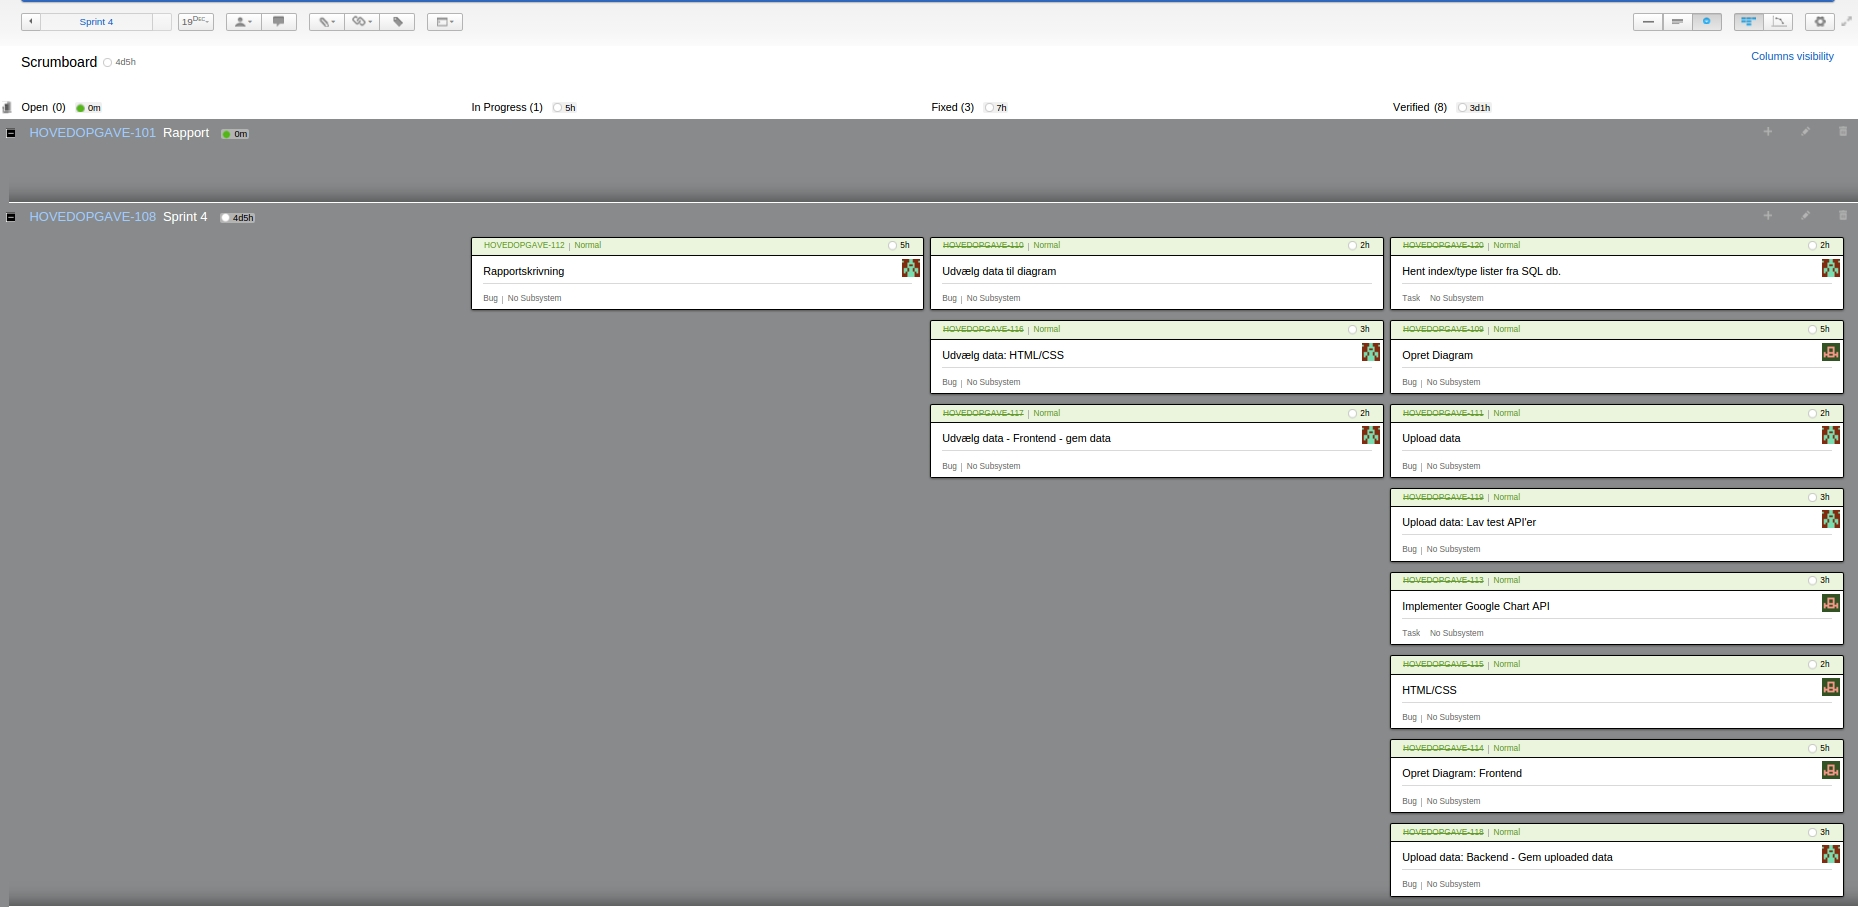
\includegraphics[scale=0.45]{Swim_lane}}
    \caption{Swim lane fra sprint 4}
    \label{fig:swim-lane}
\end{figure}
\begin{figure}[here]
    \makebox[\textwidth]{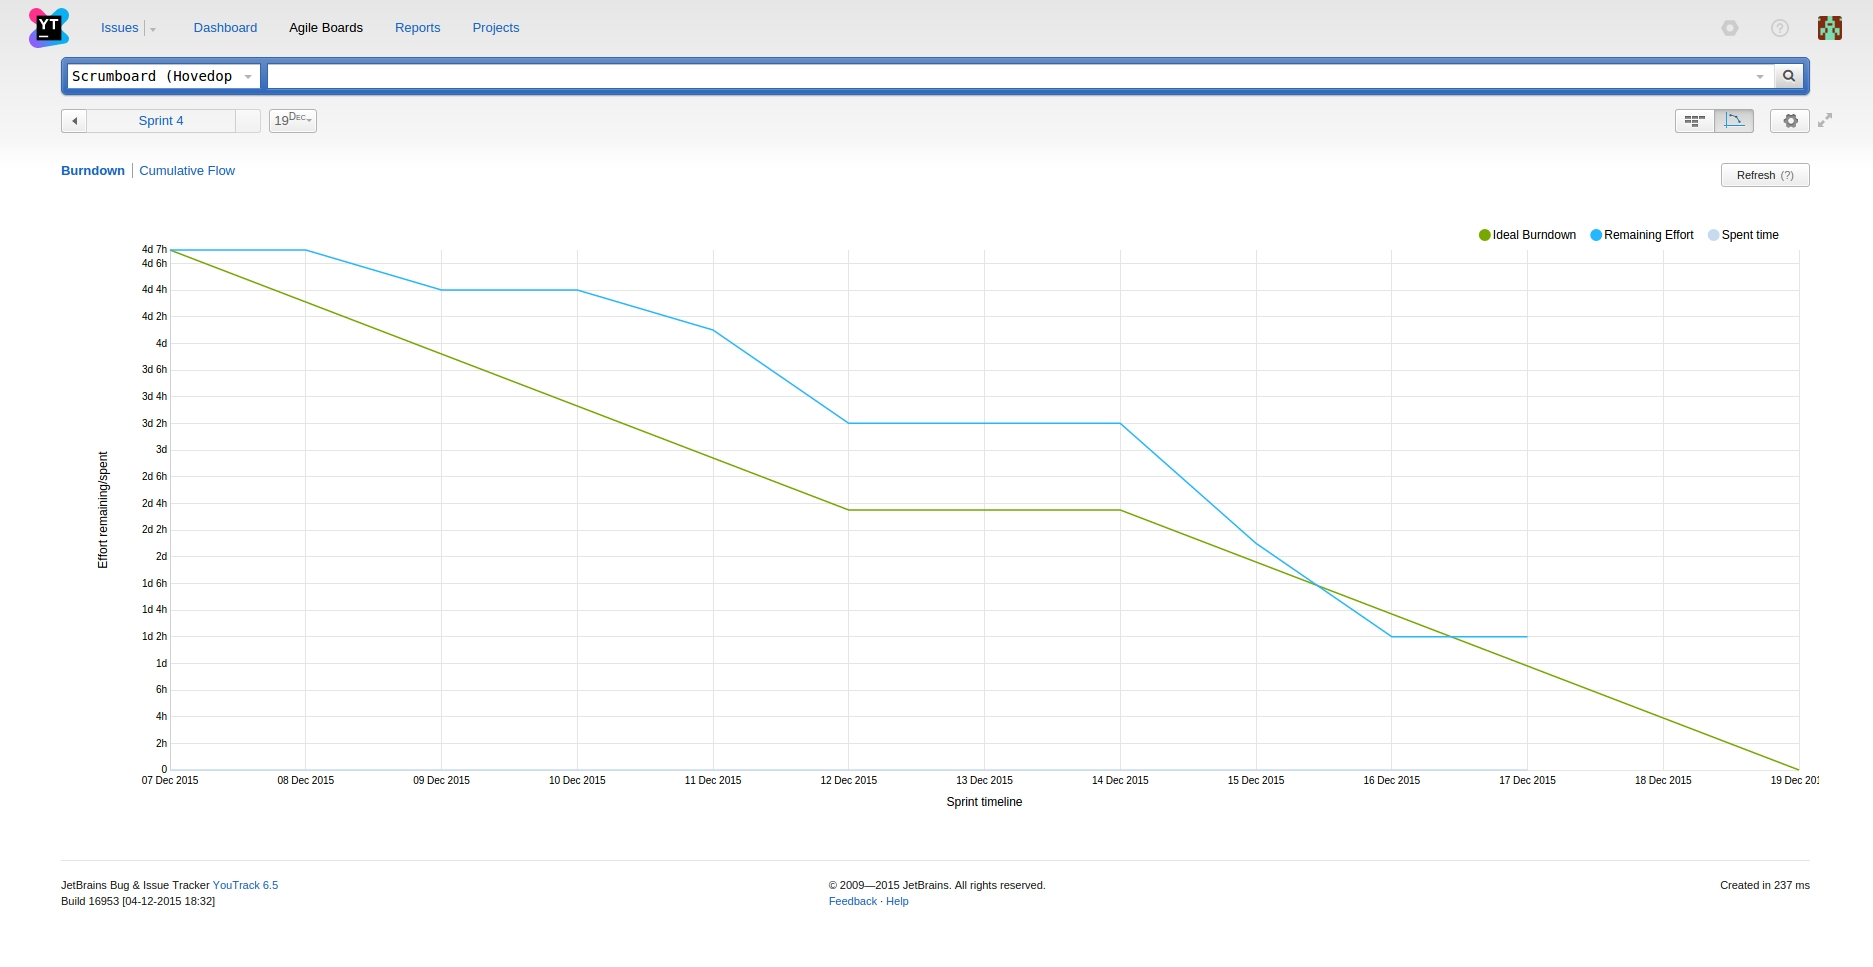
\includegraphics[scale=0.35]{Burndown_chart}}
    \caption{Burndown chart fra sprint 4}
    \label{fig:burndown-chart}
\end{figure}
\subsection{Review referater}
I dette afsnit vil vi referere de vigtigste ting fra sprint reviews i løbet af projektperioden
\subsubsection{Fredag d. 20/11}
Tilstedeværende til mødet: Mikkel, Christoffer, Michael og Peter
Vi præsenterede hvad vi havde lavet i løbet af sprintet, som primært var CRUD til håndtering af brugere. Derudover havde vi brugt meget tid på at strukturere systemet, skrive rapport, generel opsætning af teknologier, mm.
Det feedback vi fik var at vi skulle fokusere mere på at lave kernefunktionalitet til systemet, så de funktioner der var vigtige for interessenter skulle vi fokusere på i stedet for f.eks. et brugersystem.
Derudover fik nogle fingerprej om hvilken retning vi skulle gå i med projektet og hvad der var vigtigt for systemet.
Nogle punkter vi kunne tage med var,
\begin{itemize}
    \item{Pull eller push af data?}
    \item{Fokus på funktionalitet}
    \item{Vælg en sti og gør den færdig (et diagram ad gangen)}
    \item{Kig evt. på google analytics mht. hentning af data (api keys)}
    \item{Guide til upload/hentning af data}
\end{itemize}
\subsubsection{Fredag d. 4/12}
Tilstedeværende til mødet: Mikkel, Christoffer, Michael og Peter
Vi præsenterede hvad vi havde lavet i løbet af sprintet, som var Hentning og visning af data, upload af API endpoint. Derudover fortalte vi omkring vores research mht. ElasticSearch og hvordan vi havde valgt at vi vil pulle vores data fra API'er frem for at det bliver pushet til vores server. På denne måde kan vi nemmere kontrollere hvad og hvor meget data der er tilgængeligt på vores ElasticSearch server.
Det feedback vi fik var at vi skulle gøre det mere specifikt hvad der skulle uploades, så det ikke er rå data der bliver uploadet til vores server, som vi skal behandle og lave statistik data ud fra, det skal være ren statistik data der bliver uploadet. På den måde skaber det mere arbejde for dem der skal uploade, men det gør at vi kun har ren statistik tilgængelig på vores server. Dette giver ikke så mange plads problemer, da det ikke fylder specielt meget at have en dato og et tal, i forhold til en masse objekter osv. Det er primært en dato eller et tidspunkt der skal være en parameter, og så en parameter der angiver et tal eller lignende for det tidspunkt.
Derudover fik vi lidt feedback på hent og vis data, i forhold til hvordan det skal fungere når der skal laves diagrammer.
Generelt gik det meget bedre end først review, og vi var på rette vej i forhold til et mere fuldendt produkt. Generelt skal vi fokusere mere på at fortsætte i samme retning, men med små-justeringer. På denne måde kan vi virkelig få gavn af disse reviews og få noget løbende feedback fra vores interessenter.
\subsubsection{Fredag d. 17/12}
